\section{結果}
\subsection{sister(X, katsuo).}
\subsubsection{当初想定した結果(自分が望ましいと考えた結果)}
「sister(X, katsuo).」のコマンドは、「katsuo」の姉か妹である「X」を列挙するコマンドだと想定しており、
「katsuo」には、「sazae」と「wakame」の二人の「姉または妹」が存在するため、
結果は、「X=sazae;X=wakame.」のようになるのが望ましいと考えた。

\subsubsection{実行結果とその説明(2で取得したスクリーンショットを貼り付けて説明する)}
実行結果は、図\ref{graph:1}のように、「X=sazae.」と応答があった。
\begin{figure}[hbtp]
  \centering
  \caption{「sister(X, katsuo).」の実行結果}
  \label{graph:1}
  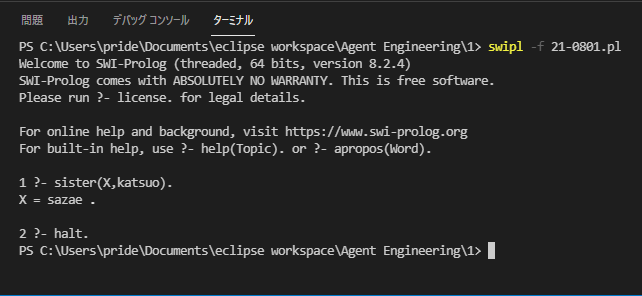
\includegraphics[scale = 0.7]{21-0801-01.png}
\end{figure}

\subsubsection{なぜそうなったかという説明。望ましくない結果であった場合はどのようにすると改善できるか}
「sister(X, katsuo).」のコマンドは、「katsuo」の姉か妹である「X」を列挙するコマンド
であるため、「katsuo」の「姉または妹」の「sazae」が出力された。
だが、実行した結果は、私が想定していた結果と違い、「X=sazae.」だけで終わってしまった。
しかし、実行したときに、「X=sazae」のように、プログラムの終了を意味する「.」が
表示されず、入力待機の時間があった。
そこで、私は「Enter」キーを押してしまったために、プログラムが終了してしまい、
「X=sazae.」だけで終わってしまったが、その入力待機の時間に「;」を入力すると、
図\ref{graph:1s}のように、私が望んだとおりの結果が出力された。
\begin{figure}[hbtp]
  \centering
  \caption{「sister(X, katsuo).」の実行中に「;」を入力した結果}
  \label{graph:1s}
  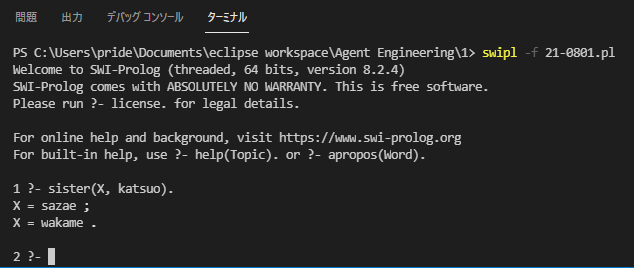
\includegraphics[scale = 0.7]{21-0801-01s.png}
\end{figure}
\clearpage

\subsection{brother(katsuo, X).}
\subsubsection{当初想定した結果(自分が望ましいと考えた結果)}
「brother(katsuo, X).」のコマンドは、「katsuo」が兄か弟である「X」を列挙するコマンドだと想定しており、
「katsuo」が、兄か弟にあたる「X」には、「sazae」と「wakame」の二人が該当するため、
結果は、「X=sazae;X=wakame.」のようになるのが望ましいと考えた。

\subsubsection{実行結果とその説明(2で取得したスクリーンショットを貼り付けて説明する)}
実行結果は、図\ref{graph:2}のように、「X=sazae.」と応答があった。
\begin{figure}[hbtp]
  \centering
  \caption{「brother(katsuo, X).」の実行結果}
  \label{graph:2}
  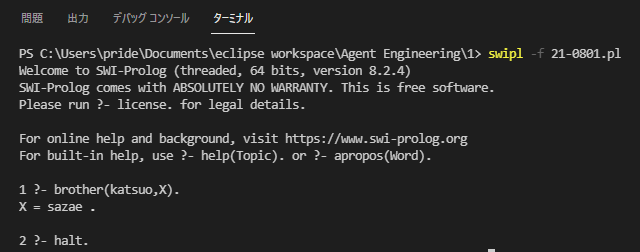
\includegraphics[scale = 0.7]{21-0801-02.png}
\end{figure}

\subsubsection{なぜそうなったかという説明。望ましくない結果であった場合はどのようにすると改善できるか}
「brother(katsuo, X).」のコマンドは、「katsuo」が兄か弟である「X」を列挙するコマンド
であるため、「katsuo」が「兄または弟」の「sazae」が出力された。
だが、実行した結果は、私が想定していた結果と違い、「X=sazae.」だけで終わってしまった。
しかし、実行したときに、「X=sazae」のように、プログラムの終了を意味する「.」が
表示されず、入力待機の時間があった。
そこで、私は「Enter」キーを押してしまったために、プログラムが終了してしまい、
「X=sazae.」だけで終わってしまったが、その入力待機の時間に「;」を入力すると、
図\ref{graph:2s}のように、私が望んだとおりの結果が出力された。
\begin{figure}[hbtp]
  \centering
  \caption{「brother(katsuo, X).」の実行中に「;」を入力した結果}
  \label{graph:2s}
  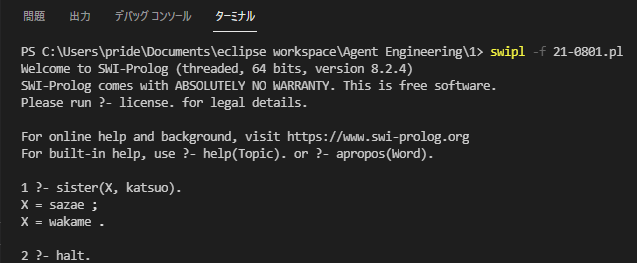
\includegraphics[scale = 0.7]{21-0801-02s.png}
\end{figure}
\clearpage

\subsection{nephew(X, wakame).}
\subsubsection{当初想定した結果(自分が望ましいと考えた結果)}
「nephew(X, wakame).」のコマンドは、「wakame」の「兄か弟または姉か妹」の息子である「X」を列挙するコマンドだと想定しており、
「wakame」の「兄か弟または姉か妹」にあたるのは、「sazae」と「katsuo」の二人が該当しており、
その中で、「sazae」には、「tara」という息子がいるので、
結果は、「X=tara.」のようになるのが望ましいと考えた。

\subsubsection{実行結果とその説明(2で取得したスクリーンショットを貼り付けて説明する)}
実行結果は、図\ref{graph:3}のように、「X=tara.」と応答があった。
\begin{figure}[hbtp]
  \centering
  \caption{「nephew(X, wakame).」の実行結果}
  \label{graph:3}
  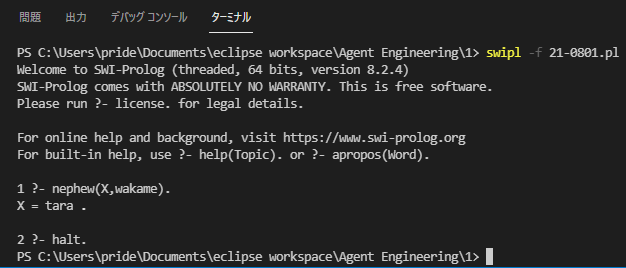
\includegraphics[scale = 1]{21-0801-03.png}
\end{figure}

\subsubsection{なぜそうなったかという説明。望ましくない結果であった場合はどのようにすると改善できるか}
「nephew(X, wakame).」のコマンドは、まず、「wakame」の「兄か弟または姉か妹」である「S」
を探索して、その「S」の男の子供を「X」として列挙する。実行結果は、私が想定していた通りで
あり、「wakame」の「兄か弟または姉か妹」である「sazae」の一人息子である「tara」
が「X」として出力された。「wakame」には、もう一人の「兄か弟または姉か妹」である「katsuo」
がいるが、「katsuo」には、息子がいなかったため、「X=tara.」で終了した。
\clearpage

\subsection{child(wakame, fune).}
\subsubsection{当初想定した結果(自分が望ましいと考えた結果)}
「child(wakame, fune).」のコマンドは、「wakame」は「fune」の子供であるかどうかを判定すると想定しており、
「wakame」は、「namihei」の子供であり、「namihei」は「fune」と結婚しているため、
結果は、「true」となるのが望ましいと考えた。

\subsubsection{実行結果とその説明(2で取得したスクリーンショットを貼り付けて説明する)}
実行結果は、図\ref{graph:4}のように、「false」と応答があった。
\begin{figure}[hbtp]
  \centering
  \caption{「child(wakame, fune).」の実行結果}
  \label{graph:4}
  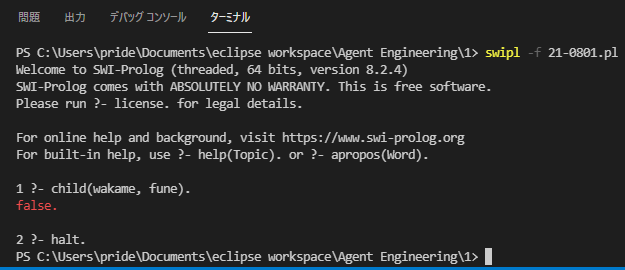
\includegraphics[scale = 1]{21-0801-04.png}
\end{figure}

\subsubsection{なぜそうなったかという説明。望ましくない結果であった場合はどのようにすると改善できるか}
「child(wakame, fune).」のコマンドで、「wakame」と「fune」は親子関係にあるはずであるが、
私の想定と違い、出力が「false」となったのは、
「child」では、「wakame」の父親である「namihei」しか定義されていないためである。
他のコマンドである、「mother」や「parent」では、「wakame」と「fune」が親子関係である
ことが定義されているため、「true」が返ってくる。
また、「child」に、「wakame」と「fune」が親子関係であることを定義することでも、
「true」が返ってくる。